% !TeX root = ../main.tex

\chapter{绪论}

\section{研究背景和意义}

\subsection{背景研究}

Hinton课题组在2012年参加ImageNet图像识别比赛时使用AlexNet\cite{AlexNet}卷积神经网络获得冠军,使得神经网络备受关注。
深度学习使用复杂的计算模型对抽象的数据表示进行学习,其能够从大量输入数据中分析并归纳出整体结构并加以分类概括。如今,在计算机视觉等领域的诸多分类问题上深度学习有着广泛的应用。
针对目标运动的分析在计算机视觉领域中大致分为三个方面:运动分割,目标检测;目标跟踪;动作识别,行为描述。

其中,目标检测不仅是计算机视觉领域需要处理的重要内容,而且它在视频追踪技术中也有着非常重要的地位。
由于图像或视频中的观测目标很可能会出现诸如被背景环境遮掩、部分细节或部分未出现在观测画面上、拍摄时的光线位置等因素导致会影响检测效果。
故目标检测在各种技术相对成熟的现在仍是诸多课题中很具有挑战性的方向,在未来会有可预见的提升空间。

遥感影像是指记录各种地物电磁波大小的胶片或照片,它主要分为航空像片和卫星相片。

随着遥感技术的飞速发展,近几年遥感图像的数量与质量得到了极大的提升。遥感图像能够描述诸如飞机、轮船、建筑设施等的地球表面的各种物体,如图\ref{RSImage}所示。

与自然场景下的普通图像相比,遥感图像有以下特点:角度是从空中拍摄;图像涵盖范围广,小目标占比很大,分布密集;旋转不变性;周围环境信息更重要;训练数据少,但单张图片像素可能极大;图片可能包含其他各种信息,如波段,地理坐标;对机器的要求更高。遥感卫星影像获取信息快,受限制条件少,更新周期短,具有用途广、效益高、动态监测等特点。遥感图像拍摄时通常为瞬时成像,能及时获取所测目标物的最新资料,不仅便于及时更新信息,而且有利于对动态变化的资料进行分析、处理和研究。

目前,遥感在农业、林业、水文、气象、军事侦察等领域有着广泛的应用,并且应用领域也在不断扩大。遥感技术有着它强大的生命力,未来有着广阔的发展、应用前景。

由于目标检测在图像处理领域起着重要作用,广泛的应用于精准农业、智能检测和地理信息系统更新等领域,在对分析和理解遥感图像以进行智能观测的强烈需求下,对于遥感图像的目标检测问题变得越来越重要。

\begin{figure}
	\center
	{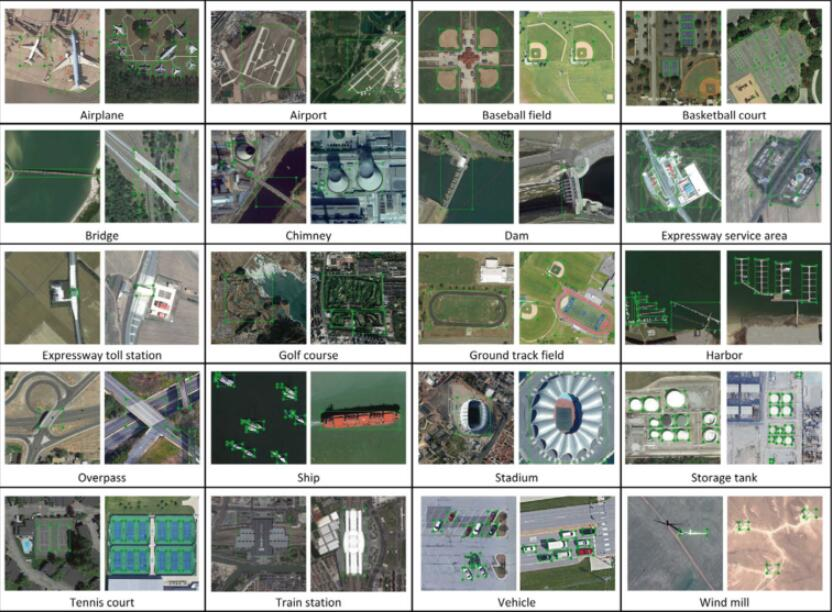
\includegraphics[width=16.64cm,height=12.25cm]{RSImage.jpg}}
	\caption{遥感图像}
	\label{RSImage}
\end{figure}


\subsection{研究意义}

目标检测,是利用计算机深度学习算法找出图像中是否存在感兴趣目标(形状、位置),同时对目标进行分类,判决目标具体是什么类别,即检测目标和识别目标。

目标检测为计算机视觉的一个热门方向,其在视频监控、机器人导航、视频监控、航空航天等许多领域有着广泛的应用。由于目标检测通过使用计算机视觉的相关算法在计算机上运行,减少了人力成本的消耗,具有着重要的现实意义。因此,近几年来目标检测逐渐成为理论与应用的研究热点。它不仅是图像处理与计算机视觉学科的重要分支,也是智能监控技术的核心组成部分;同时目标检测也是识别领域的一个基础性算法,对最近很火的人脸识别算法、视频追踪、实体分割等技术起着非常重要的作用。

由于目前遥感图像数据集有着图像数目较少、图像中研究目标的信息缺乏、图像多样性匮乏等不足之处,虽然目前已经有着成熟的高效率高准确性的基于深度学习的目标检测算法,但是对于遥感图像数据集中的识别检测还是非常困难,有着很大的发展空间。


\section{国内外研究现状}

自深度学习的概念被提出以来,其吸引了非常多的个人与企业对这个领域进行深入研究。2015年在《自然》杂志上名为《Deep Learning》\cite{Deep}的文章发表之后,深度学习在全球范围内掀起了浪潮。

Google、Amazon、Microsoft、Apple等国际大公司在深度学习方面的研究都很深入,做出的很多相关产品在日常生活中有着广泛的应用,比如Microsoft的交互机器人“Cortana”,Google的质能推荐服务,Apple的语音助手“siri”等。我国对于深度学习的研究同样也有长足的发展,很多如百度、腾讯、阿里等科技公司逐渐开始全方位多层次地涉及相关内容,并有着与国际企业并驾齐驱的势头,将该技术应用在智能设备、医疗机械、推荐系统等方面。

\subsection{传统的目标检测算法的发展}

目标检测、物体分类的研究在计算机视觉学科里有着非常重要的作用。对人来说,将看到的音频、图片上面的物体的进行分类相当简单。而计算机缺乏泛化分类的处理能力,不能理解具体目标的抽象概念;在收到输入像素信息后,并不能直接处理得到输入文件中包含哪些物体。很多时候输入的内容也会出现噪声、物体不连续、目标尺寸过小等问题,导致计算机处理分析难上加难。

传统的目标检测算法包括产生目标建议框、对每个建议框中的特征进行提取和根据特征进行分类回归三个阶段。

\paragraph{产生目标建议框}对于输入的图片,计算机只能知道具体像素点的信息,无法直接感知整体的特征。需要在原图上进行穷举建议框来预测出包含物体的建议框,即用不同大小尺度的滑动窗口依次在整张图片上进行扫描。显然,这种方法不仅运算量很大,而且大部分都在计算都是相重复的,导致了整体执行的效率极低。

\paragraph{对每个建议框中的特征进行提取}比如传统的目标检测算法中的HOG算法\cite{HOG}使用直方图统计来对物体的边缘进行编码,这样有着较强的识别表达能力,不过该算法需要人工指定特征设计,可靠性并不高。

\paragraph{根据特征进行分类回归}机器学习领域里面有着较多优秀的分类器,但是其在速度与精度方面并不能达到物体识别的要求。并且随着深度学习算法在计算机视觉学科上面优异表现的冲击,传统识别算法逐渐退出舞台。

\subsection{基于深度学习的目标检测技术发展}

从AlexNet网络在ImageNet数据集上表现出了前所未有的极好效果开始,深度学习方法便逐渐应用到了目标检测领域上。之后的几年中,各种结构的模型陆续出现,不断刷新对于如VOC、COCO等公认的标准数据集的检测准确率,性能方面也在逐渐提升。

如今,高性能与质量的目标检测算法都是基于深度学习的。最早首次使用深度学习模型来提取图像特征的R-CNN(Region-based CNN)\cite{RCNN},它的准确率达到了49.6\%,使得目标检测算法实现了划时代的进步。但是早期基于深度学习的目标检测,在生成目标建议框时也都是用滑动窗口的方式,本质上与穷举法无异,即仍未解决重复计算的问题。

为了解决冗余计算这个问题,Fast R-CNN\cite{FRCNN}被提出来了。为了合并R-CNN的训练和测试过程,Fast R-CNN在卷积层后全连接层前加了一个简化的SPP层。虽然重复计算的问题被解决了,但是其速度仍满足不了实时检测的需求。

而Faster R-CNN\cite{Faster}中的RPN(Region Proposal Networks)网络的表现要好了很多。Faster R-CNN\cite{Faster}则直接使用RPN网络来生成目标候选框。RPN网络对输入的原始图像进行处理,输出一批包含目标置信度与坐标位置信息的矩形区域。从R-CNN到Fast R-CNN再到Faster R-CNN是一个不断改进优化的过程,它使用一个深度学习的网络模型将传统目标检测的三个步骤整合起来。

随着以YOLO\cite{YOLO}和SSD\cite{SSD}方法为代表的一阶段目标检测算法的提出与优化,目标检测领域又到达了一个新的高度,它们真正的做到了实时效果。
一阶段目标检测算法在速度上有着显著的优势,并且随着模型的不断发展,一阶段的目标检测器的精度越来越高,能够达到检测需求。




\section{研究内容}

实验研究一阶段的基于anchor的神经网络和注意力机制发展在遥感图像上的应用。ASSD\cite{ASSD}是近年来结合上述两个研究点先进性网络,我们将研究与现存的一些基于深度学习的遥感图像目标检测方法相比,ASSD是否可以在速度和精度上取得一个更好的平衡。

\section{组织结构}

全文分为五章,整体组织结构如下:

第一章为绪论部分,主要介绍了现在目标检测算法研究的内容和意义所在,同时介绍了国内外的研究现状。

第二章相关技术介绍,主要介绍了本实验中利用到的各项主要概念、技术与原理;包括卷积神经网络、Resnet网络、目标检测器的分类及特点、注意力机制以及遥感图像的介绍。

第三章为本实验的网络模型ASSD的结构分析,介绍了其网络结构、候选框机制、特征融合机制与注意力单元。

第四章是本实验的实验过程与结果分析,主要介绍了本文实验的环境,实验室用的数据集以及对实验结果的评估等内容。

第五章是论文的总结与展望,总结了本文的主要工作并展望该方向今后的研究工作。

